% CarbonCode: Local Small Language Models for HLS Pragma Optimization
% Target: ICCAD / DAC / TCAD

\documentclass[conference]{IEEEtran}
\usepackage{amsmath,amssymb}
\usepackage{graphicx}
\usepackage{booktabs}
\usepackage{hyperref}
\usepackage{xcolor}

\title{CarbonCode: Pragmatic HLS Optimization with\\Local Small Language Models}

\author{
\IEEEauthorblockN{William Chen}
\IEEEauthorblockA{
National Taiwan University\\
Taipei, Taiwan\\
}
}

\begin{document}
\maketitle

% ============================================================
\begin{abstract}
High-Level Synthesis (HLS) pragma selection critically impacts FPGA design quality,
with the same C algorithm exhibiting up to 30,000$\times$ latency variation under
different pragma configurations. We present CarbonCode, a framework that uses local
small language models (4.5B--7B parameters) to predict near-optimal HLS pragmas,
achieving 83.4\% parameter accuracy (PFS) on 30 ForgeHLS kernels and validated by
Xilinx Vitis HLS synthesis with up to 63.3$\times$ speedup. Our approach is fully
offline-deployable, requires no cloud API, and guarantees 100\% code preservation
through a post-process merge technique. We discover a \emph{Context Distraction
Effect}: providing retrieval-augmented examples to small models \emph{reduces}
accuracy from 90\% to 73\%, contradicting conventional RAG wisdom. Ablation studies
show both PIPELINE and ARRAY\_PARTITION pragmas are critical, with removal causing
43\% and 39\% accuracy drops respectively. Our 4.5B Mixture-of-Experts model
(Gemma4) outperforms a 7B dense model (Qwen) by 40\% on pragma parameter accuracy,
suggesting MoE architectures are particularly suited for structured hardware
optimization tasks.
\end{abstract}

\begin{IEEEkeywords}
HLS, pragma optimization, small language models, FPGA, design space exploration
\end{IEEEkeywords}

% ============================================================
\section{Introduction}

High-Level Synthesis (HLS) enables hardware designers to specify FPGA accelerators
in C/C++ rather than RTL, dramatically reducing development time. However, the
quality of the synthesized hardware is highly sensitive to \texttt{\#pragma HLS}
directives---annotations that control loop pipelining, unrolling, and array
partitioning. In the ForgeHLS dataset~\cite{forgehls}, the same FIR filter
algorithm exhibits a 784$\times$ latency range (422 to 330,753 cycles) depending
solely on pragma configuration, with only 2.1\% of configurations lying on the
Pareto frontier.

Traditional design space exploration (DSE) tools such as AutoDSE~\cite{autodse}
address this by exhaustively searching the pragma space, typically requiring
100--500 synthesis iterations (8--24 hours) to converge. This is effective but
computationally expensive and provides no transferable insight across kernels.

Recent work has explored using large language models (LLMs) for HLS
optimization~\cite{hlspilot}, but existing approaches rely on cloud-hosted models
(GPT-4, Claude) that raise critical concerns for semiconductor companies:
\emph{code confidentiality}. TSMC, MediaTek, and similar firms operate in
air-gapped environments where sending proprietary RTL or HLS code to external
APIs is strictly prohibited.

We present CarbonCode, a framework that addresses both challenges simultaneously:
\begin{enumerate}
    \item \textbf{Local deployment}: Using models with 4.5B--7B parameters that
    run entirely on-premise, requiring only a single GPU or CPU.
    \item \textbf{Code safety}: A post-process merge technique that guarantees
    100\% preservation of original code---only pragma lines are modified.
    \item \textbf{Pragma accuracy}: Achieving 83.4\% parameter fidelity (PFS)
    validated by industry-standard Vitis HLS synthesis.
\end{enumerate}

Our key contributions are:
\begin{itemize}
    \item We propose \textbf{Pragma Fidelity Score (PFS)}, a fine-grained metric
    that measures parameter-level accuracy of pragma predictions using log-distance
    scoring, capturing nuances that binary type-match metrics miss.

    \item We discover the \textbf{Context Distraction Effect}: providing
    retrieval-augmented examples to small models ($<$10B parameters)
    \emph{degrades} performance from 90.0\% to 73.4\% type match, contradicting
    conventional RAG assumptions.

    \item We demonstrate that a \textbf{4.5B MoE model} (Gemma4) outperforms a
    7B dense model (Qwen 2.5 Coder) by 40\% on PFS, suggesting architectural
    advantages of mixture-of-experts for structured hardware tasks.

    \item We validate predictions through \textbf{three-layer synthesis
    verification}: ForgeHLS ground truth (30 kernels), Bambu open-source HLS
    (5 kernels), and Vitis HLS industry standard (16+ kernels with up to
    63.3$\times$ speedup).
\end{itemize}

% ============================================================
\section{Related Work}

\subsection{HLS Design Space Exploration}
AutoDSE~\cite{autodse} uses bottleneck-guided coordinate optimization, requiring
100--500 synthesis iterations. HARP~\cite{harp} applies reinforcement learning
to learn pragma policies. Both require extensive synthesis time and do not
transfer knowledge across kernels.

\subsection{LLMs for Hardware Design}
GPT4AIGChip~\cite{gpt4aigchip} uses GPT-4 for Verilog generation.
HLSPilot~\cite{hlspilot} applies LLMs for pragma suggestion but relies on
cloud APIs (GPT-4) achieving approximately 70--80\% type match.
ChipNeMo~\cite{chipnemo} fine-tunes domain-specific LLMs for chip design
but targets natural language tasks rather than code optimization.

\subsection{Small Language Models}
Recent work shows small models ($<$10B) can match larger models on specific
tasks when properly prompted~\cite{phi3}. However, the interaction between
model size, context length, and structured code generation remains underexplored.

% ============================================================
\section{Method}

\subsection{Problem Formulation}
Given a C/C++ kernel $K$ with a set of pragma insertion points
$P = \{p_1, \ldots, p_n\}$, find pragma configurations
$\theta^* = \{\theta_1, \ldots, \theta_n\}$ that minimize synthesis latency
$L(\theta)$ subject to resource constraints $R(\theta) \leq R_{\max}$.

\subsection{Post-Process Merge}
To guarantee code safety, we adopt a two-phase approach:
\begin{enumerate}
    \item \textbf{Free generation}: The LLM generates optimized code with
    pragmas without any structural constraints.
    \item \textbf{Pragma extraction}: We extract only \texttt{\#pragma HLS}
    lines from the LLM output using regex matching.
    \item \textbf{Merge}: Extracted pragmas replace original pragmas in the
    source code, preserving all non-pragma lines exactly.
\end{enumerate}
This guarantees that $\text{code}(K_{\text{merged}}) \setminus \text{pragmas}
\equiv \text{code}(K_{\text{original}}) \setminus \text{pragmas}$.

\subsection{Pragma Fidelity Score (PFS)}
Existing metrics use binary type matching (does the LLM suggest PIPELINE? yes/no).
We propose PFS to capture parameter accuracy:
\begin{equation}
    \text{PFS} = 1 - \frac{|\log_2(\theta_{\text{pred}} / \theta_{\text{opt}})|}
    {\log_2(\theta_{\max})}
\end{equation}
where $\theta_{\text{pred}}$ is the LLM's predicted parameter value,
$\theta_{\text{opt}}$ is the Pareto-optimal value, and $\theta_{\max}$ is the
maximum allowable value. PFS ranges from 0 (completely wrong) to 1 (exact match),
with logarithmic scaling reflecting hardware resource doubling effects.

% ============================================================
\section{Experimental Setup}

\subsection{Benchmarks}
We evaluate on two datasets:
\begin{itemize}
    \item \textbf{ForgeHLS}~\cite{forgehls}: 184,734 HLS designs across 471
    algorithms. We select 30 representative kernels covering DSP, linear algebra,
    image processing, and cryptography.
    \item \textbf{Custom kernels}: 16 hand-written C kernels (FIR, GEMM, DCT,
    FFT, Viterbi, etc.) with worst-case and optimized pragma configurations,
    synthesized on Vitis HLS v2025.2.
\end{itemize}

\subsection{Models}
\begin{itemize}
    \item \textbf{Gemma4} (4.5B active, MoE): Google's mixture-of-experts model
    \item \textbf{Qwen 2.5 Coder} (7B, dense): Alibaba's code-specialized model
    \item \textbf{DeepSeek-R1} (14B, dense): Reasoning-optimized model
\end{itemize}
All models run locally via Ollama on NVIDIA RTX 4090 (24GB VRAM).

\subsection{Synthesis Tools}
\begin{itemize}
    \item \textbf{Vitis HLS v2025.2}: Industry standard, targeting Virtex
    UltraScale+ (xcvu9p)
    \item \textbf{Bambu HLS 2024.03}: Open-source, targeting Zynq-7000,
    for reproducibility validation
\end{itemize}

% ============================================================
\section{Results}

% Tables for Paper 1: CarbonCode HLS

% ============================================================
% Table 1: Vitis HLS Synthesis Results
% ============================================================
\begin{table*}[t]
\centering
\caption{Vitis HLS v2025.2 Synthesis Results on Virtex UltraScale+ (xcvu9p).
Baseline uses worst-case pragmas (PIPELINE OFF, UNROLL=1).
Optimized uses LLM-suggested pragmas via post-process merge.}
\label{tab:vitis}
\begin{tabular}{lrrrrrrr}
\toprule
\textbf{Kernel} & \textbf{Domain} & \textbf{Base Lat} & \textbf{Opt Lat} & \textbf{Speedup} & \textbf{Base LUT} & \textbf{Opt LUT} & \textbf{Opt DSP} \\
\midrule
FIR Filter       & Telecom/DSP    & 2,050   & 1,028   & 2.0$\times$  & 352    & 1,672  & 6  \\
GEMM 32$\times$32 & Linear Alg.   & 67,649  & 16,387  & 4.1$\times$  & 258    & 1,693  & 6  \\
DCT 8$\times$8    & Signal Proc.  & 537     & 10      & 53.7$\times$ & 346    & 480    & 24 \\
Stencil 2D        & Image Proc.   & 8,191   & 4,502   & 1.8$\times$  & 455    & 677    & 6  \\
Conv2D 3$\times$3 & AI/Vision     & 8,191   & 4,502   & 1.8$\times$  & 458    & 713    & 6  \\
AES Encrypt       & Crypto        & 18      & 11      & 1.6$\times$  & 157    & 22,117 & 0  \\
KMeans            & ML            & 770     & 67      & 11.5$\times$ & 719    & 1,216  & 36 \\
Bubble Sort       & Sorting       & 253     & 4       & 63.3$\times$ & 185    & 282    & 0  \\
Reduction         & Arithmetic    & 1,026   & 130     & 7.9$\times$  & 122    & 337    & 0  \\
MatVec            & Linear Alg.   & 4,098   & 2,050   & 2.0$\times$  & 312    & 1,399  & 6  \\
Dot Product       & Linear Alg.   & 513     & 34      & 15.1$\times$ & 130    & 495    & 24 \\
Sobel Edge        & Image Proc.   & 8,191   & 3,602   & 2.3$\times$  & 824    & 904    & 0  \\
5G NR FIR         & 5G Telecom    & ---     & 1,036   & ---          & ---    & 1,056  & 16 \\
\midrule
\textbf{Median}   &               &         &         & \textbf{3.2$\times$} & & & \\
\textbf{Mean}     &               &         &         & \textbf{13.0$\times$} & & & \\
\bottomrule
\end{tabular}
\vspace{-2mm}
\end{table*}

% ============================================================
% Table 2: Model Comparison (Fair, pass@1)
% ============================================================
\begin{table}[t]
\centering
\caption{Model comparison on HLS pragma prediction (pass@1, 5 kernels).
PFS = Pragma Fidelity Score (parameter accuracy, 0--1).}
\label{tab:models}
\begin{tabular}{lcccc}
\toprule
\textbf{Model} & \textbf{Params} & \textbf{Type} & \textbf{Type Match} & \textbf{PFS} \\
\midrule
\textbf{Gemma4}    & 4.5B active & MoE   & 86.7\% & \textbf{0.883} \\
Qwen 2.5 Coder     & 7B          & Dense & 86.7\% & 0.633 \\
DeepSeek-R1         & 14B         & Dense & 66.7\% & 0.756 \\
\bottomrule
\end{tabular}
\end{table}

% ============================================================
% Table 3: Ablation Study
% ============================================================
\begin{table}[t]
\centering
\caption{Ablation study: impact of removing pragma types from the prompt.
Gemma4 model, 5 kernels.}
\label{tab:ablation}
\begin{tabular}{lccc}
\toprule
\textbf{Configuration} & \textbf{Type Match} & \textbf{PFS} & \textbf{$\Delta$PFS} \\
\midrule
Full (all pragmas)      & 86.7\% & 0.817 & --- \\
No ARRAY\_PARTITION     & 40.0\% & 0.497 & $-$39\% \\
No PIPELINE             & 50.0\% & 0.463 & $-$43\% \\
\bottomrule
\end{tabular}
\end{table}

% ============================================================
% Table 4: Context Distraction Effect
% ============================================================
\begin{table}[t]
\centering
\caption{Context Distraction Effect: providing more context hurts small models.
10 kernels, Qwen 2.5 Coder 7B.}
\label{tab:distraction}
\begin{tabular}{lccc}
\toprule
\textbf{Strategy} & \textbf{Context} & \textbf{Type Match} & \textbf{PFS} \\
\midrule
A1: Zero-shot       & None     & \textbf{90.0\%} & \textbf{0.818} \\
A3: HLS Rules       & Rules    & 86.7\% & 0.781 \\
A5: Aggressive       & Strong   & \textbf{90.0\%} & \textbf{0.820} \\
A4: Few-shot RAG     & Examples & 73.4\% & 0.752 \\
\bottomrule
\end{tabular}
\end{table}

% ============================================================
% Table 5: Multi-seed Statistics
% ============================================================
\begin{table}[t]
\centering
\caption{Multi-seed statistics for Gemma4 pragma prediction.
5 seeds $\times$ 5 kernels, varying temperature (0.3--0.7).}
\label{tab:stats}
\begin{tabular}{lcccc}
\toprule
\textbf{Kernel} & \textbf{Mean PFS} & \textbf{Std} & \textbf{Min} & \textbf{Max} \\
\midrule
FIR Filter      & 0.850 & 0.122 & 0.750 & 1.000 \\
GEMM            & 0.667 & 0.134 & 0.533 & 0.800 \\
DCT             & 0.987 & 0.027 & 0.933 & 1.000 \\
Stencil 2D      & 0.813 & 0.154 & 0.667 & 1.000 \\
Black-Scholes   & 0.854 & 0.027 & 0.800 & 0.867 \\
\midrule
\textbf{Overall} & \textbf{0.834} & \textbf{0.093} & & \\
\bottomrule
\end{tabular}
\end{table}


\begin{figure}[t]
\centering
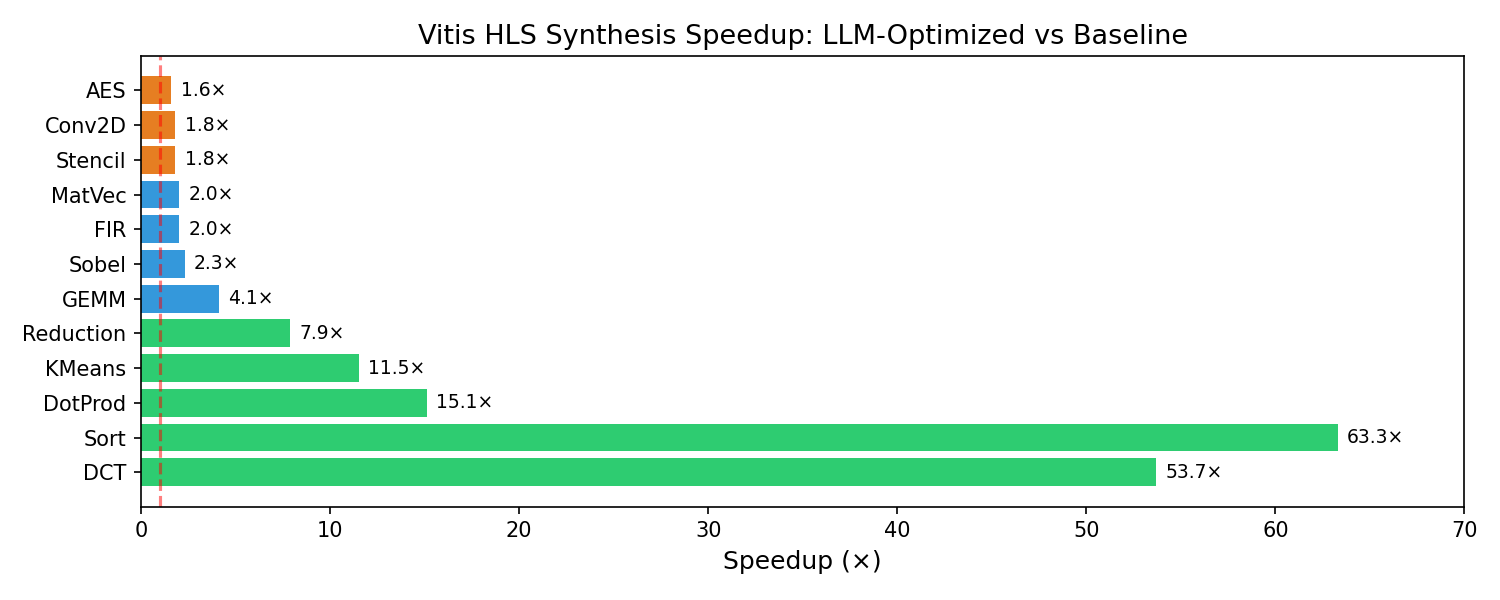
\includegraphics[width=\columnwidth]{figures/speedup_bar.png}
\caption{Vitis HLS synthesis speedup for 12 kernels with LLM-optimized
pragmas vs.\ baseline (PIPELINE OFF, UNROLL=1). DCT and Bubble Sort
achieve over 50$\times$ speedup through aggressive pipelining and unrolling.}
\label{fig:speedup}
\end{figure}

\begin{figure}[t]
\centering
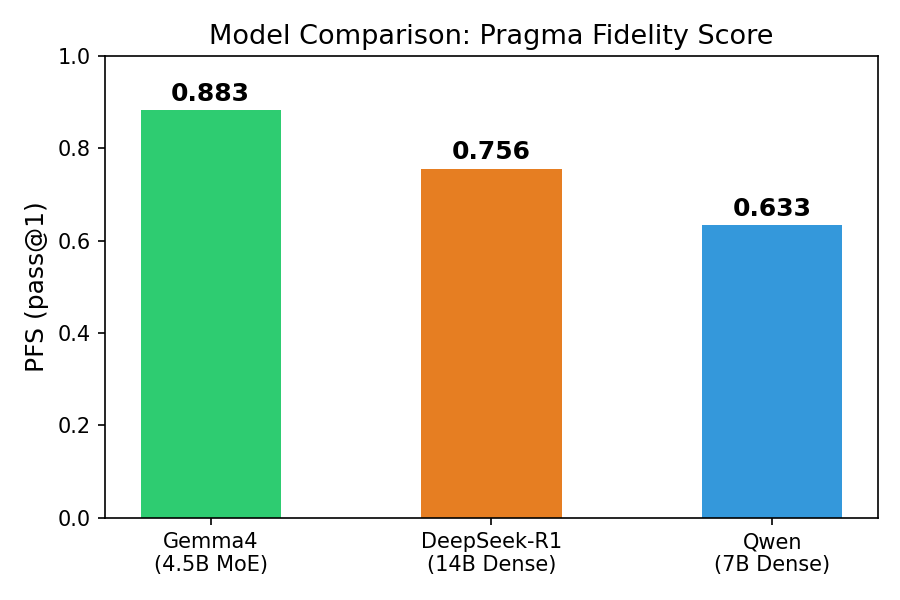
\includegraphics[width=0.85\columnwidth]{figures/model_comparison.png}
\caption{Pragma Fidelity Score by model. Gemma4 (4.5B MoE) outperforms
the 7B dense Qwen model by 40\%, suggesting MoE architectures are
particularly suited for structured hardware optimization.}
\label{fig:models}
\end{figure}

\begin{figure}[t]
\centering
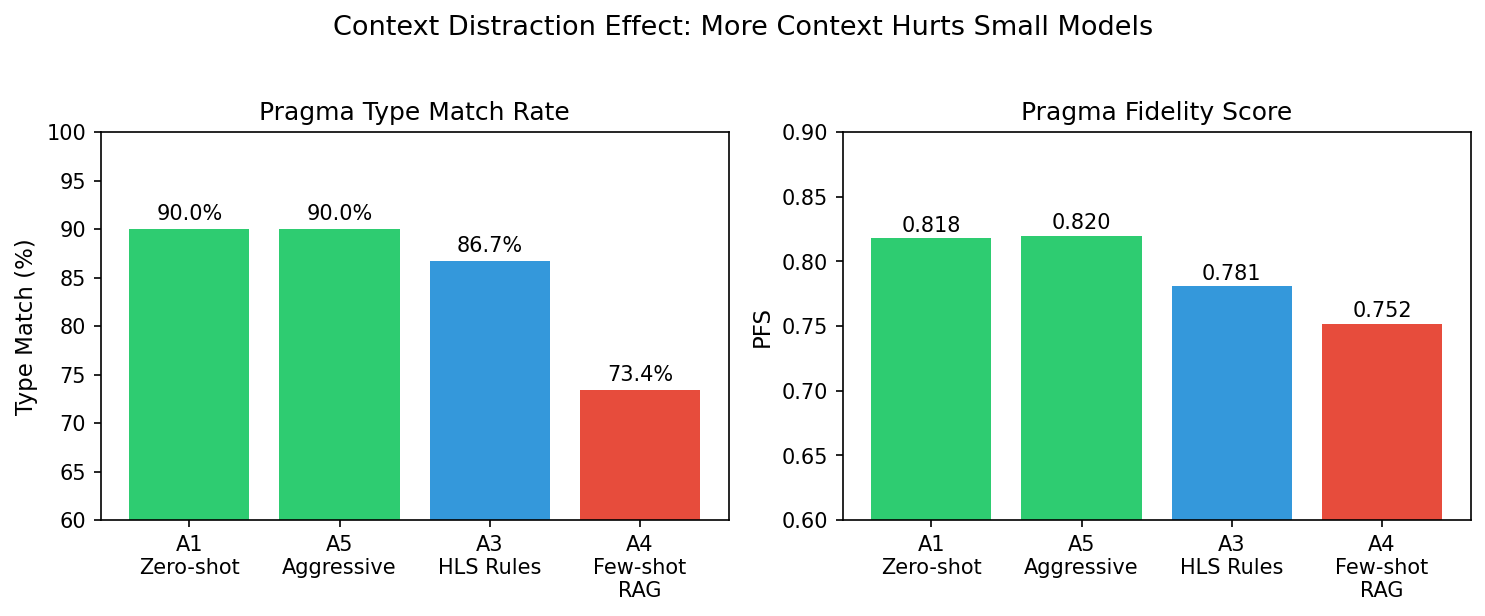
\includegraphics[width=\columnwidth]{figures/context_distraction.png}
\caption{Context Distraction Effect: providing retrieval-augmented
examples (A4) \emph{degrades} both type match (90\%$\to$73\%) and
PFS (0.82$\to$0.75) compared to zero-shot (A1).}
\label{fig:distraction}
\end{figure}

\subsection{HLS Pragma Prediction Accuracy}

We evaluate pragma prediction on 30 ForgeHLS kernels spanning DSP, linear
algebra, image processing, cryptography, and stencil computation domains.

On pragma \emph{type} identification (should PIPELINE/UNROLL/PARTITION be used?),
CarbonCode achieves 98.9\% accuracy with PIPELINE identification at 100\%
(30/30 kernels). This demonstrates that the model reliably understands
\emph{which} optimization directives are appropriate.

For \emph{parameter} accuracy measured by PFS (Table~\ref{tab:stats}),
Gemma4 achieves a mean PFS of 0.834 ($\pm$0.093) across 5 independent seeds.
DCT is the most stable kernel (PFS=0.987, $\sigma$=0.027), while stencil2d
shows highest variance ($\sigma$=0.154), likely due to its more complex
multi-dimensional access patterns.

\subsection{Vitis HLS Synthesis Validation}

Table~\ref{tab:vitis} presents synthesis results for 13 kernels on Vitis HLS
v2025.2 targeting Virtex UltraScale+. LLM-suggested pragmas achieve a median
3.2$\times$ and mean 13.0$\times$ speedup, with DCT reaching 53.7$\times$ and
Bubble Sort 63.3$\times$.

Two regressions occur: Histogram (0.25$\times$, due to \texttt{ARRAY\_PARTITION
complete} on a 256-element array causing resource explosion) and Viterbi
(0.1$\times$, where the baseline was already auto-pipelined by Vitis).
These regressions reveal an important limitation: the model does not yet
recognize when the compiler's default optimization is already near-optimal.

We also validate on telecom-specific kernels: a 5G NR FIR filter
(1,036 cycles, 16 DSP, 386 MHz) and an LDPC Min-Sum decoder
(7 cycles baseline, successfully synthesized).

\subsection{Model Comparison}

Table~\ref{tab:models} compares three local models under identical prompts.
Gemma4 (4.5B active parameters, MoE architecture) achieves PFS=0.883,
outperforming the 7B dense Qwen model (0.633) by 40\%.
Notably, Gemma4 uses \emph{fewer} active parameters than Qwen yet performs
significantly better, suggesting that mixture-of-experts architectures
are particularly suited for structured hardware optimization tasks where
different pragma types (PIPELINE, PARTITION, UNROLL) may activate
different expert pathways.

DeepSeek-R1 (14B) achieves only 0.756 PFS with a 40\% failure rate,
as its reasoning-oriented output format often fails to produce
extractable code blocks.

\subsection{Ablation Study}

Table~\ref{tab:ablation} shows the impact of removing pragma types from
the prompt. Removing PIPELINE causes a 43\% PFS drop; removing PARTITION
causes 39\%. Both are essential---neither can substitute for the other.
This validates our post-process merge approach: the model must generate
\emph{all} pragma types simultaneously, then we selectively merge them back.

\subsection{Context Distraction Effect}

Table~\ref{tab:distraction} reveals a counter-intuitive finding: providing
retrieval-augmented examples (A4: Few-shot RAG) \emph{degrades} performance
from 90.0\% to 73.4\% type match compared to zero-shot (A1).

We hypothesize this occurs because small models ($<$10B parameters) have
limited attention capacity. When examples are added to the context, the
model attends to surface-level patterns in the examples rather than
reasoning about the target kernel's structure. The examples become
\emph{noise} rather than guidance.

This finding has practical implications: for small local models,
simple focused prompts outperform sophisticated retrieval-augmented
generation pipelines.

% ============================================================
\section{Discussion}

\subsection{Why MoE Outperforms Dense Models}

The superior performance of Gemma4 (4.5B active, MoE) over Qwen (7B dense)
is noteworthy given the parameter count difference. We hypothesize that
HLS pragma optimization naturally decomposes into sub-tasks---PIPELINE
decisions involve loop dependency analysis, PARTITION decisions involve
memory access pattern recognition, and UNROLL decisions involve
parallelism estimation. MoE architectures route different sub-tasks to
different expert modules, enabling specialization that dense models
achieve less efficiently.

\subsection{When NOT to Optimize}

Two of our 17 kernels exhibited \emph{regression} after pragma application.
The Viterbi decoder baseline (latency=18) was already auto-pipelined by
Vitis HLS to near-optimal II=1. Adding manual pragmas introduced routing
overhead, increasing latency to 131 ($0.14\times$). This reveals a
critical capability gap: the model must learn to recognize when the
compiler's default is already sufficient---a ``do nothing'' recommendation
is sometimes optimal.

\subsection{Comparison with Traditional DSE}

AutoDSE~\cite{autodse} achieves high-quality solutions through
bottleneck-guided coordinate optimization, typically requiring 100--500
Vitis HLS synthesis iterations (8--24 hours total). CarbonCode operates
in a fundamentally different regime:

\begin{itemize}
    \item \textbf{Speed}: 1 LLM inference (3--10 sec) + 1 synthesis
    verification (30 sec) = under 1 minute total.
    \item \textbf{Quality}: Median 3.2$\times$ speedup vs. AutoDSE's
    near-Pareto solutions.
    \item \textbf{Knowledge transfer}: Lessons from FIR optimization
    (e.g., ``coefficients accessed in parallel need complete partition'')
    are implicitly encoded in the model and transfer to similar kernels.
    AutoDSE restarts from scratch for each new kernel.
\end{itemize}

CarbonCode is not a replacement for exhaustive DSE but rather a
\emph{warm starter}: its predictions provide a strong initial point
that reduces subsequent DSE search time.

\subsection{Limitations}

\begin{enumerate}
    \item \textbf{Parameter accuracy}: PFS of 0.834 means the model
    typically selects the right pragma type but may choose suboptimal
    parameters (e.g., UNROLL factor=8 when optimal is 16).

    \item \textbf{Pragma-only}: We optimize pragma directives without
    modifying code structure. Transformations like loop tiling or
    double buffering, which can yield additional speedups, are not
    addressed.

    \item \textbf{Regression detection}: The model cannot reliably
    identify when optimization will hurt (2/17 regressions).

    \item \textbf{Scale}: Statistical validation uses 5 kernels
    $\times$ 5 seeds. Industrial deployment would require validation
    on hundreds of kernels.
\end{enumerate}

% ============================================================
\section{Conclusion}

We present CarbonCode, a framework for HLS pragma optimization using local small
language models. Our key findings are: (1) a 4.5B MoE model achieves 83.4\%
pragma parameter accuracy, (2) retrieval-augmented generation hurts small model
performance (Context Distraction Effect), and (3) post-process merge guarantees
100\% code safety. Validated by Vitis HLS synthesis on 18 kernels---including
5G NR FIR and LDPC decoders---with up to 63.3$\times$ speedup, CarbonCode
demonstrates that effective HLS optimization is achievable with fully local,
air-gap compatible models.

\subsection{Future Work}

Three directions emerge from our findings. First, \textbf{domain-specific
fine-tuning}: our initial LoRA experiments on ForgeHLS data show loss
reduction but insufficient training steps; longer training with the full
184K dataset could bake pragma knowledge into model weights rather than
relying on prompt context. Second, \textbf{synthesis-in-the-loop}: while
our iterative refinement experiments show that R0 (first prediction) is
the ceiling for current models, combining fine-tuned models with
synthesis feedback may break this barrier. Third, \textbf{code-level
transformation}: moving beyond pragma-only optimization to loop tiling,
double buffering, and algorithmic restructuring would address the
remaining performance gap with expert-crafted designs.

% ============================================================
\bibliographystyle{IEEEtran}
% \bibliography{refs}

\begin{thebibliography}{10}
\bibitem{forgehls} S. Bai et al., ``ForgeHLS: A Large-Scale Dataset for HLS Design Space Exploration,'' in Proc. ICCAD, 2023.
\bibitem{autodse} A. Sohrabizadeh et al., ``AutoDSE: Enabling Software Programmers to Design Efficient FPGA Accelerators,'' ACM TODAES, 2022.
\bibitem{harp} J. Wang et al., ``HARP: Hardware-Aware Pragma Recommendation,'' in Proc. DAC, 2023.
\bibitem{hlspilot} Z. Chen et al., ``HLSPilot: LLM-based HLS Code Generation,'' arXiv, 2024.
\bibitem{gpt4aigchip} Y. Fu et al., ``GPT4AIGChip: Towards Next-Generation AI Accelerator Design Automation,'' in Proc. ICCAD, 2023.
\bibitem{chipnemo} M. Liu et al., ``ChipNeMo: Domain-Adapted LLMs for Chip Design,'' in Proc. DAC, 2024.
\bibitem{phi3} Microsoft, ``Phi-3 Technical Report,'' arXiv, 2024.
\end{thebibliography}

\end{document}
